% !TeX program = LuaLaTeX
% !TeX encoding = UTF-8
% !TeX spellcheck = pt_PT
% !TeX hyphenation = pt_PT

% Latex style for final reports and dissertations (Instituto Politécnico de Beja)
% Version 0.8.1, 2021/10/01
% Author: João Paulo Barros, joao.barros@ipbeja.pt
% Com contribuições de Henrique Água-Doce, Nuno Mourinho e Raul Carvalho.

%para texto em Português verdadeiro (pt_PT)
\documentclass[PT]{ipbeja-format}
%for text in real English (also change the magic comment locale to en_GB)
%\documentclass[]{ipbeja-format}

% !TeX program = LuaLaTeX
% !TeX encoding = UTF-8
% !TeX spellcheck = pt_PT
% !TeX hyphenation = pt_PT

% Para preencher
\newcommand{\ESCOLA}{Escola Superior de Tecnologia e Gestão}
\newcommand{\CURSO}{Licenciatura em Engenharia Informática}

\newcommand{\TITULO}{Relatório de Estágio}
\newcommand{\SUBTITULO}{Desenvolvimento em Backend na Optiply}

\newcommand{\NOMEALUNO}{Gonçalo Candeias Amaro}
\newcommand{\LOCAL}{Beja, Portugal}

\newcommand{\ORIENTADORIPBEJAA}{Gonçalo Fontes}
% se existir segundo orientador do IPBeja, retirar o comentário da linha seguinte
%\newcommand{\ORIENTADORIPBEJAB}{Colocar o nome do(a) segundo(a) docente orientador(a), se existente}

%se for um estágio deve ser retirado o comentário da linha seguinte e indicar o orientador na entidade de acolhimento do estágio
\newcommand{\ORIENTADORENTIDADE}{Fábio Belga}

%Completar e comentar um dos seguintes dois \newcommand
%\newcommand{\DECLARACAOPROJETO}{Relatório de projeto de fim de curso apresentado na\linebreak \ESCOLA{} do Instituto Politécnico de Beja}
\newcommand{\DECLARACAO}{Relatório de estágio, realizado na Optiply, apresentado na\linebreak \ESCOLA{} do Instituto Politécnico de Beja}

% retirar comentário e preencher se existente
%\newcommand{\DEDICATORIA}{ texto a colocar }
%LOL! NOPE, NIGGA. Do you want me to act like Snoop Dogg in the Hollywood star award? "I wanna thank me for believing in me."

\usepackage[]{hyperref}
\hypersetup{hidelinks,hypertexnames=true}

\begin{document}
\pagenumbering{roman}
\setcounter{page}{1}
\folhacapa % 2.1 das normas
\folharosto % 2.3 das normas
%%%%%%%%%%%%%%%%%%%%%%%%%%%%%%%%%%%%%%%%%%%%
\frontmatter % parte inicial

\clearpage
\chapter{Resumo}
\section*{\textit{\TITULO}\\  {\small{\textit{\SUBTITULO}}}}

\textit{Este relatório consiste na representação e documentação do decorrer do Estágio Profissional, realizado como parte integrante e conclusiva da Licenciatura em Engenharia informática pela Escola Superior de Tecnologia e Gestão do Instituto Politécnico de Beja.}

\textit{O Estágio Profissional desenvolveu-se na Optiply, em Évora, no ano lectivo de 2021/2022, tendo como objectivo favorecer a integração e consolidação, no contexto da pratica, os conhecimentos teóricos adquiridos durante o decorrer da Licenciatura.}

\textit{O objetivo primordial do estágio seria o de integração no mundo do trabalho. A ideia de se estagiar na Optiply veio no sentido de propiciar ao estudante um primeiro contacto com a área do desenvolvimento em Backend, e a possibilidade de se desenvolver pessoalmente num ambiente de trabalho que seja compatível com o que se pretende fazer.}

\textit{As atividades foram desenvolvidas tendo sempre em conta os objetivos inicialmente delineados e que se propôs atingir para a função do estagiário, que foram: treino inicial via cursos do Udemy, o desenvolvimento de um projeto, planificação e implementação do mesmo.}

\textit{Este referido projecto foi um projecto de desenvolvimento de Backend, que foi desenvolvido em Java, utilizando o framework Micronaut, ligado a uma base de dados Postgres, e que foi desenvolvido num ambiente de desenvolvimento local usando containers Docker.}

\textit{A aprendizagem durante o estágio foi efectiva e perceptível, na medida em que se desenvolveram diversas atividades que proporcionaram a aquisição e o desenvolvimento de diferentes competências técnicas e organizacionais.}

\textbf{Palavras-chave}: \textit{Estágio, Profissional, Postgres, Backend, Desenvolvimento, Docker, Java, Micronaut}.

\clearpage
\chapter{Abstract}
\section*{\textit{\TITLE}\\  {\small{\textit{\SUBTITLE}}}}

\textit{This report consists in the representation and documentation of the coursework of the Curricular Internship, carried out as a part of the Bachelor Degree in Computer Science at the School of Technology and Management of the Polytechnic Institute of Beja.}

\textit{The Internship was carried out at Optiply, in Évora, in the year of 2020/2021, with the aim of improving the integration and consolidation of the acquired knowledge, in a professional context, the knowledge academically acquired throughout the Degree.}

\textit{The primordial objective of the internship was to improve the integration in the world of work. The idea of being interned at Optiply came from the idea of improving the student's first contact with the area of development in Backend, and the possibility of developing personally in an environment of work that is compatible with what the student intends to do after the completion of this Degree.}

\textit{The activities were developed taking into account the objectives initially outlined and that were: initial training via Udemy courses, the development of a project, planning and implementation of it.}

\textit{This project was the development of a Microservice, using Java, with the Micronaut framework, linked to a Postgres database, and it was developed in a local development environment using Docker containers.}

\textit{The learning was effective and perceptible, in the measure in which the activities that were developed that provided the acquisition and the development of different technical and organizational competences.}

\textbf{Keywords}: \textit{Internship, Professional, Postgres, Backend, Development, Docker, Java, Micronaut}.


\clearpage
\indicegeral
%\clearpage
%\indicedefiguras % Remover se houver menos de 5 figuras
%\clearpage
%\indicedetabelas % Remover se houver menos de 5 tabelas
%\clearpage
%\indicedelistagens % Remover se houver menos de 5 listagens

% No caso de se verificar "um número significativamente elevado de abreviaturas e siglas" deve retirar-se o
% comentário da linha seguinte e preencher o ficheiro parte-inicial/abreviaturas.tex
\chapter{Abreviaturas, Siglas e Acrónimos}

\begin{longtable}{p{.15\textwidth} p{.85\textwidth}}

  API    & Application Programming Interface                           \\
  CLI    & Command Line Interface                                      \\
  CRUD   & Create Read Update and Delete                               \\
  DAO    & Data Access Object                                          \\
  HTTP   & Hypertext Transfer Protocol                                 \\
  IPBeja & Instituto Politécnico de Beja                               \\
  JDBC   & Java Database Connectivity                                  \\
  JDK    & Java Development Kit                                        \\
  jOOQ   & jOOQ Object Oriented Querying \textit{(Acrónimo Recursivo)} \\
  JSON   & JavaScript Object Notation                                  \\
  POJO   & Plain Old Java Object                                       \\
  REST   & Representational State Transfer                             \\
  SDK    & Software Development Kit                                    \\
  SQL    & Structured Query Language                                   \\
  URI    & Uniform Resource Identifier                                 \\
  URL    & Uniform Resource Locator
\end{longtable}


%%%%%%%%%%%%%%%%%%%%%%%%%%%%%%%%%%%%%%%%%%%%
\mainmatter  \pagestyle{ruled} % parte principal
\pagenumbering{arabic}

\chapter{Introdução}
\label{intro}

Este presente relatório tem como objetivo apresentar o decorrer do estágio profissional e as consequências ou resultados do mesmo, o qual ocorreu no período de 02/03/2022 a 02/06/2022, na cidade de Évora, Portugal. O estágio foi hospedado pela \href{https://optiply.nl/}{Optiply}, que é uma empresa de gestão inteligente de \textit{stocks} dos produtos e serviços de lojas online, cujo orientador (Fábio Belga) é o \textit{Team Leader/Tech Lead}, que gere todo o processo de desenvolvimento e gestão do projeto.

O meu papel como estagiário foi um de treino para desenvolvimento em backend com um pequeno projeto, um \textit{microservice} que realiza a gestão de especificações de lojas online. Este projeto envolveu variadas tecnologias e paradigmas de trabalho e de programação, os quais passam por diversas etapas de desenvolvimento, testes e documentação, mas no que toca à gestão e organização de projeto foi de escolha livre, ou seja, eu geria o meu tempo e o projeto à minha vontade sem vigilância ou controlo. O qual, admitindo a verdade, não geri o meu tempo de qualquer forma, apenas os objetivos de projeto em sí, num estilo primitivo de Kanban.

Com a leitura deste relatório, pretendo que gradualmente se expanda e detalhe o referido no paragrafo anterior, e que seja possível compreender o que foi aprendido e o que foi desenvolvido.

\chapter{A Empresa}
\label{cap2}

\section{Caracterização}

\lipsum

\section{Organização e Comunicação}

\lipsum

\section{Tech Stack}

\lipsum

\section{Produto}

\lipsum

\chapter{\textit{Onboarding}}\label{cap3}

Aqui descrevo o meu breve processo de Onboarding. O qual passou pelo primeiro dia onde foi a parte administrativa, e posteriormente a parte formativa onde durante duas semanas estive a ser preparado para o projeto.

\section{O que é Onboarding?}

Em linhas gerais, onboarding trata-se de um processo para integrar o novo membro à equipa, cultura e forma de operação da empresa, com o objetivo de assegurar a adaptação e a retenção deste profissional.

É o processo de integração de novos empregados numa empresa, para que eles possam obter os conhecimentos, as habilidades e os comportamentos necessários a fim de efetivamente se tornarem parte da equipa.

Envolve várias etapas, que podem ser conjuntas ou separadas, como orientação, supervisão, acompanhamento e treinamento, por exemplo.

\section{Fase Administrativa}

Chamo de fase administrativa ao primeiro dia de estágio, este dia passou pela introdução informal do local de estágio, as regras de trabalho, as normas de segurança e o que é necessário para o bom desenvolvimento do projeto.

Foi também neste dia que me foi atribuído a conta empresarial (backend da Google), com email, senha e perfil de acesso, como também o que esta conta oferece (tal como drive, sheets, etc).

Essa conta base serve também para login na conta da Atlassian, onde tenho acesso a todas as ferramentas de estágio, como o Jira, Confluence, Bitbucket, etc.

Finalmente foi feita uma reunião, comigo e com todos os outros estagiários (três alunos da Universidade de Évora, sendo que um também é um estagiário de Backend), para nos passar à fase formativa, onde estarei a desenvolver competências base para o projeto.

\newpage

\section{Fase Formativa}

Esta fase teve uma duração base de duas semanas. Aqui foi-nos doado três cursos do \href{https://www.udemy.com/}{Udemy}, gradualmente e squencialmente dependendo do progresso do estagiário.

Estes cursos tinham como objetivo ajudar ao estagiário a desenvolver competências para o projeto que será desenvolvido, o qual reflete as competências que o estagiário deve possuir para poder trabalhar no backend da empresa que está a trabalhar.

O primeiro curso foi \href{https://www.udemy.com/course/build-reactive-restful-apis-using-spring-boot-webflux/}{\textit{``Build Reactive MicroServices using Spring WebFlux/SpringBoot''}}, que têm como objetivo ensinar a fazer backends de serviços, ou micro serviços em Spring, mas com uma particularidade: usar \href{https://spring.io/reactive}{Spring WebFlux} que é a implementação da \href{https://spring.io/}{Spring} do \href{https://projectreactor.io/}{Project Reactor}. Isto permite fazer uma API reativa, ou seja, uma API que é capaz de receber requisições e retornar respostas de forma assíncrona e com a menor latência possível.

\begin{figure}[!hbt]
  \centering
  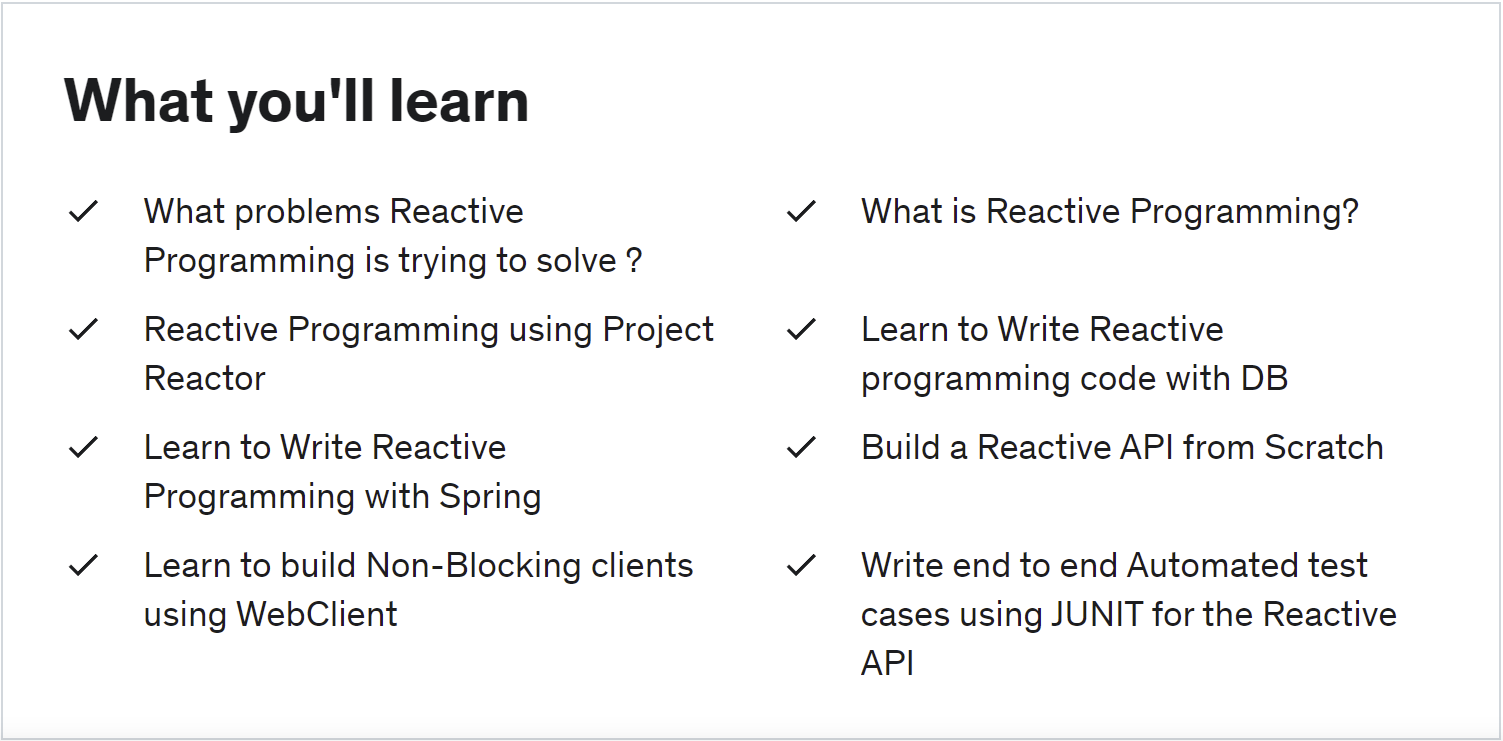
\includegraphics[width=14cm]{figuras/udemy1.png}
  \caption{Conteúdo do curso \textit{``Build Reactive MicroServices using Spring WebFlux/SpringBoot''} do \href{https://www.udemy.com/}{Udemy}}
  \label{fig:udemy1}
\end{figure}
\FloatBarrier

Seguidamente foi-me destacado o \href{https://www.udemy.com/course/grpc-the-complete-guide-for-java-developers/}{\textit{``Microservices with gRPC [Java + Spring Boot + Protobuf]''}}, que é um curso com o objetivo de ensinar ao estagiário a desenvolver \textit{microservices} com \href{https://grpc.io/}{gRPC} em \href{https://jdk.java.net/}{Java} usando \href{https://developers.google.com/protocol-buffers}{Protocol Buffers}, ou seja, um serviço que usa a implementação de RPC da \href{https://abc.xyz/}{Google} e usa o \href{https://developers.google.com/protocol-buffers}{Protocol Buffers} para o transporte de dados. Isto têm a vantagem de ser um serviço de baixo custo, e alta velocidade de comunicação.

\begin{figure}[!hbt]
  \centering
  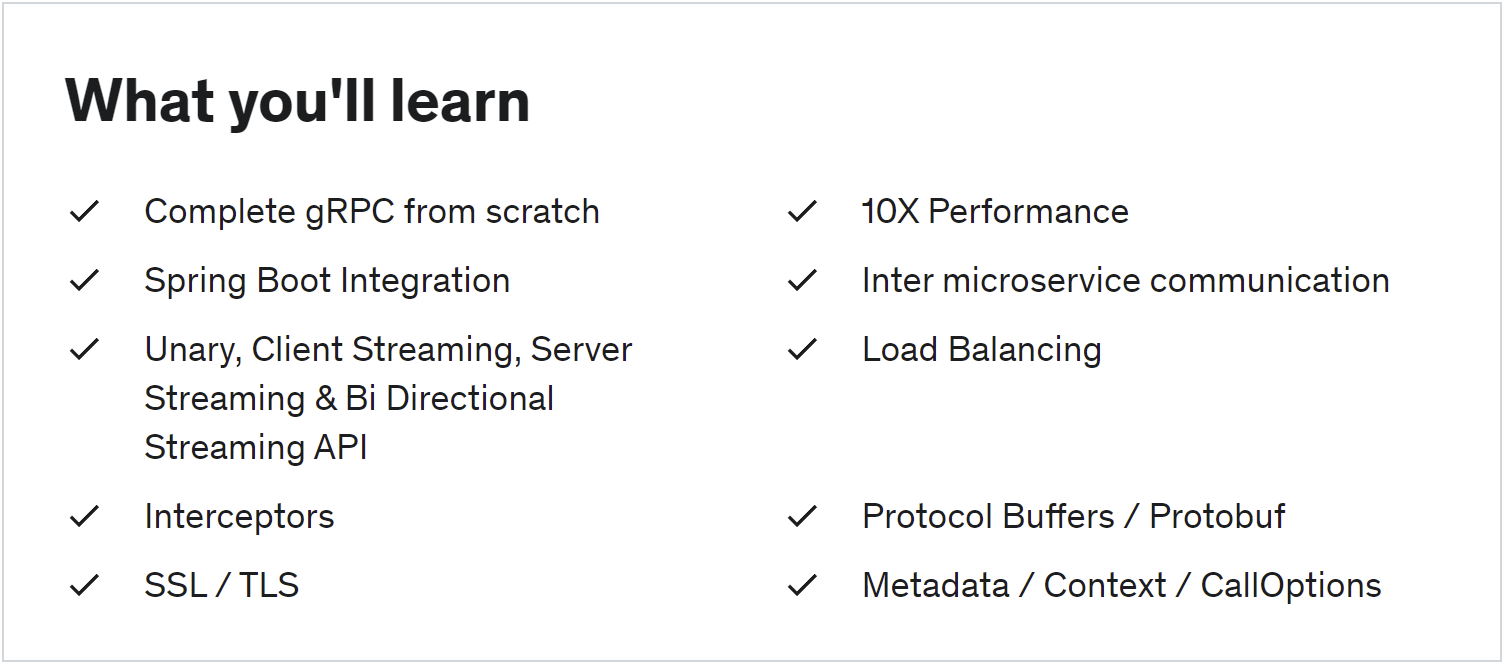
\includegraphics[width=14cm]{figuras/udemy2.png}
  \caption{Conteúdo do curso \textit{``Microservices with gRPC [Java + Spring Boot + Protobuf]''} do \href{https://www.udemy.com/}{Udemy}}
  \label{fig:udemy2}
\end{figure}
\FloatBarrier

O ultimo curso foi o \href{https://www.udemy.com/course/learn-micronaut/}{\textit{``Learn Micronaut - cloud native microservices with Java''}}, que nos mostra como fazer \textit{microservices} em Micronaut, um framework de \href{https://jdk.java.net/}{Java}, como o Spring mas com o objetivo de ser mais leve, modular e escalável. Este curso também passa pela integração do \href{https://kafka.apache.org/}{Apache Kafka}, um \textit{message broker} que permite a comunicação entre \textit{microservices} e como exportar o projeto para um \textit{native binary} e como usar o \href{https://www.graalvm.org/}{GraalVM}, que é uma JVM de nova geração, mais leve e mais rápida que também suporta outras linguagens de programação.

\begin{figure}[!hbt]
  \centering
  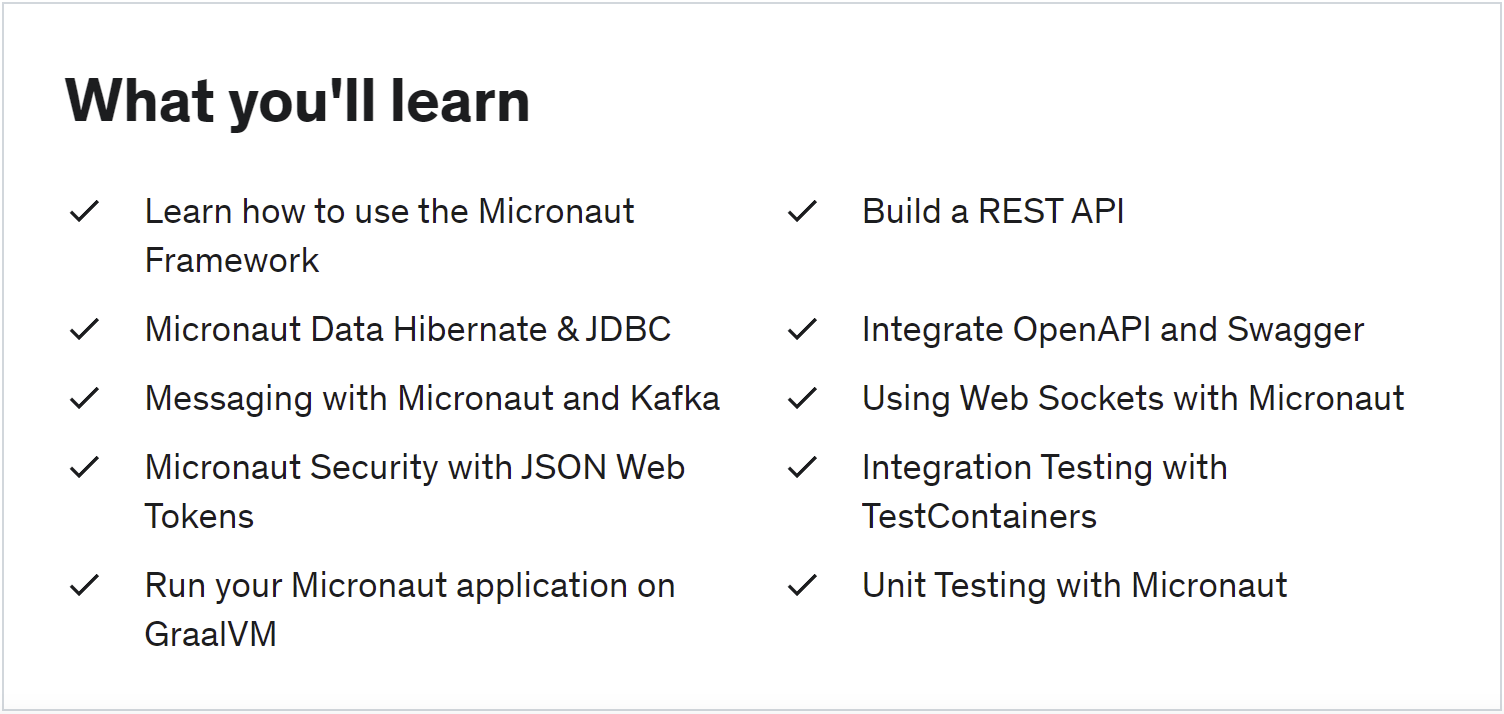
\includegraphics[width=14cm]{figuras/udemy3.png}
  \caption{Conteúdo do curso \textit{``Learn Micronaut - cloud native microservices with Java''} do \href{https://www.udemy.com/}{Udemy}}
  \label{fig:udemy3}
\end{figure}
\FloatBarrier

\chapter{Desenvolvimento do projeto}\label{cap4}

Este capítulo descreve o projeto atribuído no estágio e o seu desenvolvimento. Sendo que este capítulo será o mais longo, mas consequentemente o mais importante e o mais complexo.

\section{Introdução}

Como anteriormente referido foi me destacada a tarefa de Implementação de um projeto no estágio. Este projeto consiste em um software que permite a gestão das especificações de Webshops.

Estas Webshops são, como o nome indica, as lojas online as quais são clientes da Optiply. Estas lojas online são responsáveis por fornecer os produtos que os clientes compram e a Optiply é responsável por fornecer a gestão inteligente dos produtos em stock.

O trabalho foi recebido num \textit{.pdf}, numa reunião de video-conferencia, com o coordenador do estágio (Fábio Belga), o seu subordinado (André Figueira)que ficou encarregado de orientar os estagiários de Backend, e nós (eu, Gonçalo Amaro e o estagiário da universade de Évora, José Azevedo), após a nossa fase formativa do \textit{Onboarding} descrita no capítulo anterior.

Assim, as primeiras secções deste capítulo servem como uma apresentação do equivalente à minha introdução ao projeto.

\section{Objetivos}

O objetivo descrito deste projeto é desenvolver um microserviço que permita a gestão das especificações de Webshops, já o verdadeiro objetivo deste projeto é fornecer treino ao estagiário nas tecnologias da \textit{Tech Stack} da empresa, ou pelo menos num dos projetos da mesma.

\newpage

Essa \textit{Tech Stack} referida é a seguinte:

\begin{itemize}
  \item Micronaut: Framework de desenvolvimento de microserviços.
  \item Java: Linguagem de programação.
  \item Gradle: Sistema de gestão de dependências e tarefas.
  \item jOOQ: Framework de código-fonte para acesso a bases de dados.
  \item Flyway: Framework de migração de bases de dados.
  \item PostgreSQL: Sistema de bases de dados.
  \item Junit5 (Spock também é aceitável): Framework de testes.
  \item Mockito: Framework de auxiliar a testes via simulação.
\end{itemize}

Voltando ao objetivo escrito do projeto (desenvolver um microserviço que permita a gestão das especificações de Webshops), o objetivo é desenvolver uma RESTful API que permita gerir as especificações de Webshops.

Para isso temos de saber que cada Webshop têm um conjunto de especificações, as quais são:

\begin{itemize}
  \item \textit{URL:} URL da loja online, têm validação e requer protocolo na URL;
  \item \textit{Handle:} identificador único da loja online;
  \item \textit{Interest Rate:} taxa de juros que a loja online paga, 20\% é o valor por defeito;
  \item \textit{Service Level Categories:} categorias de níveis de serviço que a loja têm, são três categorias (A,B e C) e as suas somas requerem ser iguais a 100\%;
  \item \textit{Contact Email List:} lista de emails de contacto da loja online, têm validação;
  \item \textbf{Extra:} \textit{Settings:} configurações da loja online:
    \begin{itemize}
      \item \textit{Enable Multi Supplier:} permite múltiplos fornecedores;
      \item \textit{Enable Run Jobs:} permite execução de tarefas;
      \item \textit{Currency:} moeda da loja online em ISO-4217;
    \end{itemize}
\end{itemize}

Sendo que as ultimas especificações (as \textit{Settings}) são Extras, ou seja, não são obrigatórias, mas foram implementadas.
\newpage

Essa API tem um determinado conjunto de tarefas a cumprir as quais são:

\begin{itemize}
  \item Obter uma única Webshop;
  \item Obter várias Webshops:
    \begin{itemize}
      \item Deve ser capaz de ordenar e filtrar por qualquer campo da tabela;
      \item Só é necessário ordenar por um único campo. Os resultados devem ser consistentes com cada pedido. (Se ordenar por Taxa de Juros, como pode-se garantir que os mesmos resultados sejam obtidos em todos os pedidos?)
      \item Só é necessário filtrar por um único campo. Os filtros suportados são:
        \begin{itemize}
          \item ``:'' significa \textit{Igual}. Exemplo: handle:optiply
          \item ``\%'' significa \textit{ILIKE} (semelhante, \textit{case-insensitive}).\\Exemplo: handle\%optiply
          \item \textbf{Extra:} ``>'' significa \textit{Maior Que}. Exemplo: interestRate>20
          \item \textbf{Extra:} ``<'' significa \textit{Menor Que}. Exemplo: interestRate<20
        \end{itemize}
    \end{itemize}
  \item Apagar uma única Webshop.
  \item Criar uma única Webshop.
  \item Atualizar qualquer campo da Webshop.
  \item \textbf{Extra:} Filtrar por múltiplos campos.
  \item \textbf{Extra:} Criar múltiplas Webshops.
  \item \textbf{Extra:} Obter as configurações da Webshop.
  \item \textbf{Extra:} Atualizar as configurações da Webshop.
\end{itemize}

Tendo sempre em conta que os resultados devem ser idempotentes e no seu estado mais recente e que os pedidos HTTP retornam:

\begin{itemize}
  \item Criar deve retornar 201.
  \item Obter e Atualizar devem retornar 200.
  \item Apagar deve retornar 204.
  \item Qualquer pedido deve retornar 404 se a loja não existir.
  \item Qualquer outro erro interno deve retornar 500 (Erro Interno).
\end{itemize}

Esta lista (tradução do que está no \textit{.pdf} recebido, que está também no \hyperref[ap1]{Apêndice I}), é bastante extensa, mas é bastante simples para entender o que é.

No entanto é estupidamente obscura a segunda intenção da lista, esta era a lista implícita de \textit{endpoints} da API\@.

O qual inicialmente não vendo uma lista de \textit{endpoints} explicita nem uma mera referência na reunião, a primeira iteração do trabalho usei os \textit{endpoints} que eu achava mais convenientes para o trabalho. Escusado será dizer, que tive de os refazer após a primeira receção de \textit{feedback}.

\newpage

\section{Implementação}

\subsection{Pré-Requisitos}

Para começar a implementar a API, precisamos de um conjunto de ferramentas. Essas ferramentas passam por um JDK (um SDK de Java), otimamente algo aberto e conforme os standards de \href{https://openjdk.org/}{OpenJDK}, o qual usei \href{https://docs.aws.amazon.com/corretto/latest/corretto-17-ug/downloads-list.html}{Amazon Corretto}, visto à sua licença aberta e gratuita, multiplataforma e vem com suporte de longo prazo que incluirá melhorias de desempenho e correções de segurança.

Para gestão de pacotes e tarefas, precisamos de um gestor de pacotes, o qual usei o \href{https://gradle.org/}{Gradle}, e como um dos meus computadores de trabalho usa \href{https://www.microsoft.com/pt-pt/software-download/windows10} em vez de \href{https://archlinux.org/download/}{Linux}, a instalação do \href{https://gradle.org/}{Gradle} sem um gestor de pacotes e alteração do path, dá-nos jeito usar um IDE que trate desses assuntos, o qual foi-me recomendado (e usado): \href{https://www.jetbrains.com/idea/}{IntelliJ IDEA} da \href{https://www.jetbrains.com/}{JetBrains}.

Para hospedar a base de dados e o projeto, numa pequena rede de containers interna, foi instalado o \href{https://www.docker.com/}{Docker} no \textit{desktop} \href{https://www.microsoft.com/pt-pt/software-download/windows10}{Windows} (e usado o \href{https://podman.io/}{Podman} no portátil \href{https://archlinux.org/download/}{Linux}, pelo simplesmente facto de já o ter instalado previamente).

No entanto ainda nos falta algo bastante importante. Nomeadamente, algo quer faça o Bootstrap do projeto em \href{https://micronaut.io/}{Micronaut}, para isso temos variadas opções:

\begin{itemize}
  \item Ir ao o \href{https://micronaut.io/launch}{Micronaut Launch Website}
  \item Usar o \href{https://micronaut.io/download/}{Micronaut CLI} \href{https://micronaut-projects.github.io/micronaut-starter/latest/guide/index.html}{em que temos aqui a documentação}
  \item Fazer \href{https://curl.se/}{curl} à API do \href{https://micronaut.io/}{Micronaut} Launch \href{https://launch.micronaut.io/create/default/com.optiply.project.webshop?lang=JAVA&build=GRADLE&test=JUNIT&javaVersion=JDK_17&features=jackson-databind&features=kubernetes-reactor-client&features=properties&features=flyway&features=jdbc-hikari&features=jooq&features=postgres&features=r2dbc&features=testcontainers&features=lombok&features=mockito&features=openrewrite&features=asciidoctor&features=logback&features=reactor&features=security-jwt&features=problem-json&features=jackson-xml}{https://launch.micronaut.io/create/default}
\end{itemize}

\subsection{Inicio do Projeto}

No meu caso em especifico foi-me fornecido um repositório privado no \href{https://bitbucket.org/}{BitBucket}, o qual apenas me foi necessário fazer uma \textit{fork}. O estado desse repositório e da \textit{fork} pode ser visto no neste \href{https://github.com/CatKinKitKat/MicronautJooqPostgresREST/tree/07d359ce933dde634f176dc95bf5ac1b3e4bc93d}{\textit{commit}} (\href{https://github.com/CatKinKitKat/MicronautJooqPostgresREST}{num repositório meu} do \href{https://github.com/}{GitHub}, onde no projeto o adicionei como segunda origem, para backup).

Esta diretoria de projeto nos atribuída, pessoalmente achei que era maior e mais complicada que o necessário, talvez esta seja única e o que varia são os projetos que a usam. Com isso em conta eu decidi, fazer uma redução ao projeto, para que ficasse mais simples de trabalhar e não houvessem pacotes ou funcionalidades que não fossem necessárias. Isto pode ser observado neste \href{https://github.com/CatKinKitKat/MicronautJooqPostgresREST/commit/3c71d709599662436ae13cf9dcf609a5ca5464e3}{\textit{commit}} (o qual descrição reflete o meu estado mental sobre determinada observação).

Após a redução, o projeto ficou com apenas dois subprojetos para o Gradle gerir, um que contem a aplicação em sí e o outro que trata dos repositórios/classes de transações à base de dados. O numero de pacotes externos e funcionalidades foi reduzido para o mínimo necessário, esses incluíram: \href{https://flywaydb.org/}{Flyway}, \href{http://fasterxml.com/}{Jackson}, \href{https://www.jooq.org/}{jOOQ}, \href{https://junit.org/junit5/}{JUnit}, \href{https://logback.qos.ch/}{Logback}, \href{https://projectlombok.org/}{Lombok}, \href{https://site.mockito.org/}{Mockito}, \href{https://jdbc.postgresql.org/}{Postgres}, \href{https://r2dbc.io/}{R2DBC} e \href{https://projectreactor.io/}{Reactor}.

\newpage

\subsubsection{Detalhes sobre as tecnologias}

\paragraph{\href{https://flywaydb.org/}{Flyway}\\}

O \href{https://flywaydb.org/}{Flyway} é um framework de migrações de bases de dados, que é usado para gerênciar as migrações de bases de dados de projetos Java. Funciona de maneira semelhante às migrações nativas do ASP.NET Core.

Este pacote adiciona essas capacidades a tarefas do Gradle, como o \textit{flywayMigrate} e \textit{flywayInfo}. A migrações são feitas através de um ficheiro de migrações, que é um ficheiro de SQL, dentro da diretoria de migrações (\textit{PROJECT\_ROOT/src/main/resources/db/migrations}), com a versão em que a migração deve ser executada e dois \textit{underscores}.

\paragraph{\href{http://fasterxml.com/}{Jackson}\\}

O \href{http://fasterxml.com/}{Jackson} é um framework de serialização de objetos, que é usado para serializar objetos em JSON.

A serialização é um processo de transformação de um objeto em um JSON, e a deserialização é o processo de transformação de um JSON em um objeto.

Isto é feito principalmente através de um objeto \textit{ObjectMapper}, que é um objeto que implementa a interface \textit{com.fasterxml.jackson.databind.ObjectMapper}.

\paragraph{\href{https://jooq.org/}{jOOQ}\\}

O \href{https://jooq.org/}{jOOQ} é um framework de código-fonte de código-aberto, que é usado para gerir a base de dados. Este funciona de maneira semelhante às operações do Entity Framework Core para ASP.NET Core, sendo que este abstrai as operações de SQL em wrappers programáticos.

\paragraph{\href{https://junit.org/junit5/}{JUnit}\\}

O \href{https://junit.org/junit5/}{JUnit} é um framework de testes, que é usado para gerênciar os testes de unidades. Usado muito na disciplina de Programação Orientada a Objetos.

\paragraph{\href{https://logback.qos.ch/}{Logback}\\}

O \href{https://logback.qos.ch/}{Logback} é um framework de logging, que é usado para gerir os logs de um projeto, com o foco em abstrair o uso de logs ao mais simples possível. É o sucessor do \href{https://log4j.org/}{Log4j}, que foi alvo de uma vulnerabilidade recentemente.

No Windows devemos alterar uma configuração: a desativação do JANSI, que não funciona com alguns Locales, em especial os que o Windows usa.

\paragraph{\href{https://projectlombok.org/}{Lombok}\\}

O \href{https://projectlombok.org/}{Lombok} é um framework de código-fonte de código-aberto, que é usado para gerir a criação de classes de objetos através de anotações. Com estas anotações, abstraímos o código, evitamos repetição e automatizamos muito o processo desenvolvimento.

Por exemplo a anotação \textit{@Getter} faz com que o Java crie automaticamente os getters. Ou, a anotação \textit{@Data} faz com que o Java crie automaticamente os getters, setters, equals, hashCode, toString e clone.

\paragraph{\href{https://site.mockito.org/}{Mockito}\\}

O \href{https://site.mockito.org/}{Mockito} é um framework auxiliar de testes, que é usado para gerir os mocks de objetos. Os mocks são objetos que são usados para simular o comportamento de objetos realmente existentes.

Com os mocks, podemos testar objetos que ainda não existem, como um objeto de um repositório de dados, ou um objeto de um serviço. Como também isolamos o comportamento dos objetos, evitamos que os objetos sejam alterados durante o teste ou para testar apenas o comportamento do que comunica com o mesmo.

\paragraph{\href{https://jdbc.postgresql.org/}{PostgreSQL}\\}

O \href{https://jdbc.postgresql.org/}{PostgreSQL} é um driver JDBC, que é usado para conectar a bases de dados PostgreSQL. Um driver JDBC é um driver que permite ao Java a comunicação com bases de dados.

PostgreSQL é o tipo de base de dados usado no projeto.

\paragraph{\href{https://r2dbc.io/}{R2DBC}\\}

O \href{https://r2dbc.io/}{R2DBC} é um driver de conexão à base de dados, mas contrariamente ao anterior este permite fazer transações reativas como as do Project Reactor ou do RxJava.

\paragraph{\href{https://projectreactor.io/}{Reactor}\\}

O \href{https://projectreactor.io/}{Reactor} é um framework de eventos, que é usado para gerir eventos e criar aplicações reativas. Uma aplicação reativa é uma aplicação que é executada em um fluxo de eventos.

\subsection{Paradigma de Programação}

Programação reativa é o acto de programar para trabalhar com fluxos de dados assíncronos. Isto é importante devido o crescimento da Internet e a demanda enorme de dados em tempo real. Esta programação precisa de ser dinâmica, ou seja; diferente das formas tradicionais de desenvolvimento.

Nas formas tradicionais de programar/desenvolver, de modo \textbf{muito} genérico, cria-se variadas tarefas e elas comunicam-se em tempos pré-determinados, com respostas pré-determinadas, são ``rígidas'', seguem regras diretas.

Isto funciona e continua a ser utilizada até hoje, entretanto esta ``lógica'' não é compatível com as necessidades de alguns serviços atuais e os seus inúmeros clientes e dados. Na programação reativa isto ocorre de uma forma semelhante, mas mais inteligente, interligada em paralelo, sem seguir uma ordem cronológica e linear.

\newpage

Os pilares da programação reativa são:

\begin{itemize}
  \item \textbf{Elástico:} Reage à demanda/carga: aplicações podem fazer uso de múltiplos núcleos e múltiplos servidores;
  \item \textbf{Resiliente:} Reage às falhas; aplicações reagem e se recuperam de
    falhas de software, hardware e de conectividade;
  \item \textbf{Message Driven:} Reage aos eventos (event driven): em vez de compor
    aplicações por múltiplas threads síncronas, sistemas são compostos de gerenciadores de eventos assíncronos e não bloqueantes;
  \item \textbf{Responsivo:} Reage aos usuários: aplicações que oferecem interações
    ricas e ``tempo real'' com usuários.
\end{itemize}

\subsection{Estrutura do Projeto}

A estrutura do projeto, como dito anteriormente, foi uma modificação do herdado da estrutura inicial vinda do repositório oferecido para \textit{forking}. Este projeto consitis de um projeto Gradle com três subprojetos: um pacote com classes entendidas de Monos, um pacote para o core do projeto, e um pacote para os repositórios que tratam das transações com a base de dados.

Sendo que as classes eram apenas \textit{MonoVoid}, \textit{MonoFalse} e \textit{MonoTrue} que simplesmente implementavam a interface \textit{Mono} e retornavam um valor booleano (ou nenhum), decidi cortá-las visto que não trazem quais quer nova funcionalidade ao projeto e não me custa escrever \textit{Mono<Boolean>} e retornar um valor booleano.

Com isto, a estrutura do projeto foi alterada para um projeto Gradle com dois subprojetos.

\subsection{Metodologia de desenvolvimento}

Foi-me notificado que o projeto seria desenvolvido de forma livre, sem qualquer metodologia de desenvolvimento. No entanto, sendo eu um alguém novo na area e a trabalhar remotamente, decidi que é extremamente importante arranjar um ambiente de desenvolvimento que me permita trabalhar, ponto. Por isto, decidi referir às estratégias de gestão de projeto ensinadas na disciplina de Engenharia de Software, como o \textit{Scrum} e o \textit{Kanban}.

Sabendo que a empresa onde estou usa \textit{Scrum}, ponderei usar o mesmo e as ferramentas disponíveis no \href{https://www.atlassian.com/}{Atlassian} como \textit{Jira} e \textit{Confluence}; mas acabei por decidi usar uma estratégia menos rígida, o \textit{Kanban}.

\newpage

\subsubsection{Kanban}

Para o meu projeto, a estratégia de desenvolvimento foi o \textit{Kanban}, ou pelo menos uma forma primitiva do mesmo. Expandindo, foi feito um quadro de tarefas divididas em cinco colunas: \textit{Tarefas}, \textit{Por aprender}, \textit{Por implementar} \textit{Por testar} e \textit{Terminadas}.

A metodologia de trabalho começava por ir identificando tarefas, se muito complexas dividi-las em pequenas tarefas e julgando a minha capacidade de as fazer. Colocando na coluna respetiva e depois trabalhando de acordo com o estado do quadro.

Este quadro infelizmente já não está acessível, pois a conta empresarial já foi fechada.

\subsubsection{Nota sobre a escolha}

Na minha opinião subjetiva, a escolha do \textit{Kanban} sobre \textit{Scrum}, foi uma boa decisão, visto que o \textit{Scrum} é um padrão mais rígido e linear, havendo a (extra) necessidade em criar \textit{user-stories} e em definir \textit{sprints}. Já o \textit{Kanban} é um padrão mais flexível, tanto por ter menos etapas para organizar como por ter um quadro de tarefas menos \textit{standard} e mais flexível.

\subsection{Testes}

Para testar o software, foi recomendado uma mistura de \textit{JUnit} e \textit{Mockito} ou usar \textit{Spock}. Estes testes foram feitos dentro do subprojeto principal, e foram divididos em duas partes:

\begin{itemize}
  \item \textit{Testes de unidade}
  \item \textit{Testes de integração}
\end{itemize}

Houve também uma secção chamada \textit{shared}, onde havia um conjunto de classes que orientava o pacote do \textit{TestContainers} e o seu \textit{container} de teste \textit{PostgreSQL}.

Noto que uma dos requerimentos do projeto era que um pacote do Gradle, chamado JaCoCo e que verifica a percentagem de código testado, fosse incluído no projeto e o resultado mínimo obtido fosse de 80\%. O que foi feito e entregue, com 82\% na entrega final e que houve uma altura que foi entregue com uns 100\% de coverage (na secção seguinte 4.3.6 saberão porquê), no então noto também que este relatório refere-se principalmente ao estado da entrega final.

\subsubsection{Testes de unidade}

Os testes de unidade são testes que testam uma unidade do software, isto quer dizer que testam algo em isolamento do resto do software. Este tipo de testes permitem verificar o correto funcionamento daquela especifica classe ou função, assim permitir identificar (ou excluir da procura) \textit{bugs} ou erros no software.

Foram feitos testes de unidade para as classes dos modelos (os objetos com que comunicamos) e para as classes de serviços.

\subsubsection{Testes de integração}

Os testes de integração são testes que testam o funcionamento do software como um todo. Este tipo de testes permitem verificar o correto funcionamento do software ou permitir identificar se existe algum \textit{bug} no software, sabendo também se esse erro está na integração das unidades se em conjunto com testes de unidade sem testes falhados.

Foi feita uma serie de testes de integração para a classe do \textit{controller}, que é responsável por receber os \textit{requests} à API e assim testando o funcionamento da API num todo.

\subsection{\textit{Feedback}}

O \textit{feedback} sobre o desenvolvido seria feito sob pedido via Slack ao responsável sobre os estagiários de backend, o André Figueira.

De forma concreta eu obtive dois sets de \textit{feedbacks}:

\begin{itemize}
  \item \textit{Feedback} da primeira entrega
  \item \textit{Feedback} da segunda entrega (final)
\end{itemize}

\subsubsection{\textit{Feedback} da primeira entrega}

Este foi o \textit{Feedback} mais volumoso, que combinou comentário sobre \textit{Clean Code} e os conceitos \textit{SOLID}, comentário sobre os verbos dos métodos \textit{HTTP} e comentário sobre ler as inferências do \textit{.pdf} do projeto.

Começando de trás para a frente, o primeiro comentário foi sobre os \textit{endpoints}. Ou seja, as ações que o software pode realizar, descritas no documento, inferem os endpoints que o software deve ter e não algo que apenas os satisfaça, lembrar o que foi dito no final da secção 4.2.

Seguinte, os caminhos da URI, para os simplificar o mais possível, não precisam de conter os verbos das ações que fazem, visto que sendo ações CRUD, descritas facilmente com os métodos HTTP (GET, PUT, POST, DELETE), podem e devem ser cortados ao máximo.

Exemplo: \texttt{\textbf{HTTP DELETE ->} http://localhost/remove/\{id\}} passar para\\\texttt{\textbf{HTTP DELETE ->} http://localhost/\{id\}}.

Por último, e não menos importante, os conceitos \textit{SOLID} devem ser seguidos ao máximo independentemente do que achamos que vai ser o rumo do software. Isto porquê? Eu achei que visto que não iriam haver mais do que uma interface de comunicação com o software, sendo apenas necessário um \textit{controller} que serve a comunicação REST HTTP, não seria necessário uma outra classe com o \textit{business logic}, ou seja uma classe de serviço onde \textit{controllers} iriam buscar. Isto estava errado mesmo que a lógica sobre esta decisão não estivesse muito errada. O software deve separar o \textit{business logic} do \textit{controller} o mais possível e o software deve ser extensível.

\subsubsection{\textit{Feedback} da segunda entrega (final)}

O \textit{feedback} desta entrega foi muito mais simples, visto que todos os pontos anteriores foram corrigidos, o \textit{feedback} foi simplesmente que o software estava satisfatório com o que foi pedido se bem que a documentação poderia ter sido um pouco mais extensa.

\chapter{Projeto desenvolvido}\label{cap5}

Este capitulo descreve em detalhe o funcionamento do projeto desenvolvido durante o decorrer do estágio.

\section{Funcionamento}

\subsection{Descrição geral}

O \textit{Webshop Service Specification} é uma RESTful API reactiva, que consiste em gerir as especificações de Webshops, ou seja um microserviço reactivo. Este microserviço recebe pedidos HTTP e retorna uma resposta JSON com o resultado, nomeadamente uma Webshop ou uma caraterística da mesma.

Sendo esta API reactiva, ela emprega o uso de \textit{threading} (divisão de tarefas em subprocessos) para poder executar variados pedidos em simultâneo, o mais depressa possível. No entanto esses processos concorrentes e assíncronos requerem um outro nível de cuidado e atenção no que toca à integridade e idempotência dos dados requeridos.

As relações empregues por uma aplicação reactiva são os padrões de \textit{Publisher/Subscriber}, onde um pedido, ou uma transação, é uma mensagem enviada pela fonte desses dados, chamada de um \textit{Publisher} e a sua receção, ou seja onde os dados são consumidos, é encarregado pelo(s) \textit{Subscriber(s)}. Se um desses pedidos for uma mensagem com varias subscrições ao longo do tempo, devemos alterar o \textit{scheduling}, que gere as filas de processos e acessos.

Com isto podemos dizer que os \textit{endpoints} desta API são \textit{Subscribers} e o serviço transacional que comunica diretamente com os dados da base de dados é o nosso \textit{Publisher}. Este tipo de acessos reactivos à base dados requer um outro tipo de mecanismo de processo de transações SQL, o qual deve ser também reactivo de modo a que a base de dados seja vista e funcione com um \textit{Publisher} e seja configurável a sua propagação.

\newpage

Pegando na excelente descrição anterior, o funcionamento deste microserviço pode ser reduzido ao seguinte \textit{flowchart}:

\begin{figure}[!hbt]
        \centering
        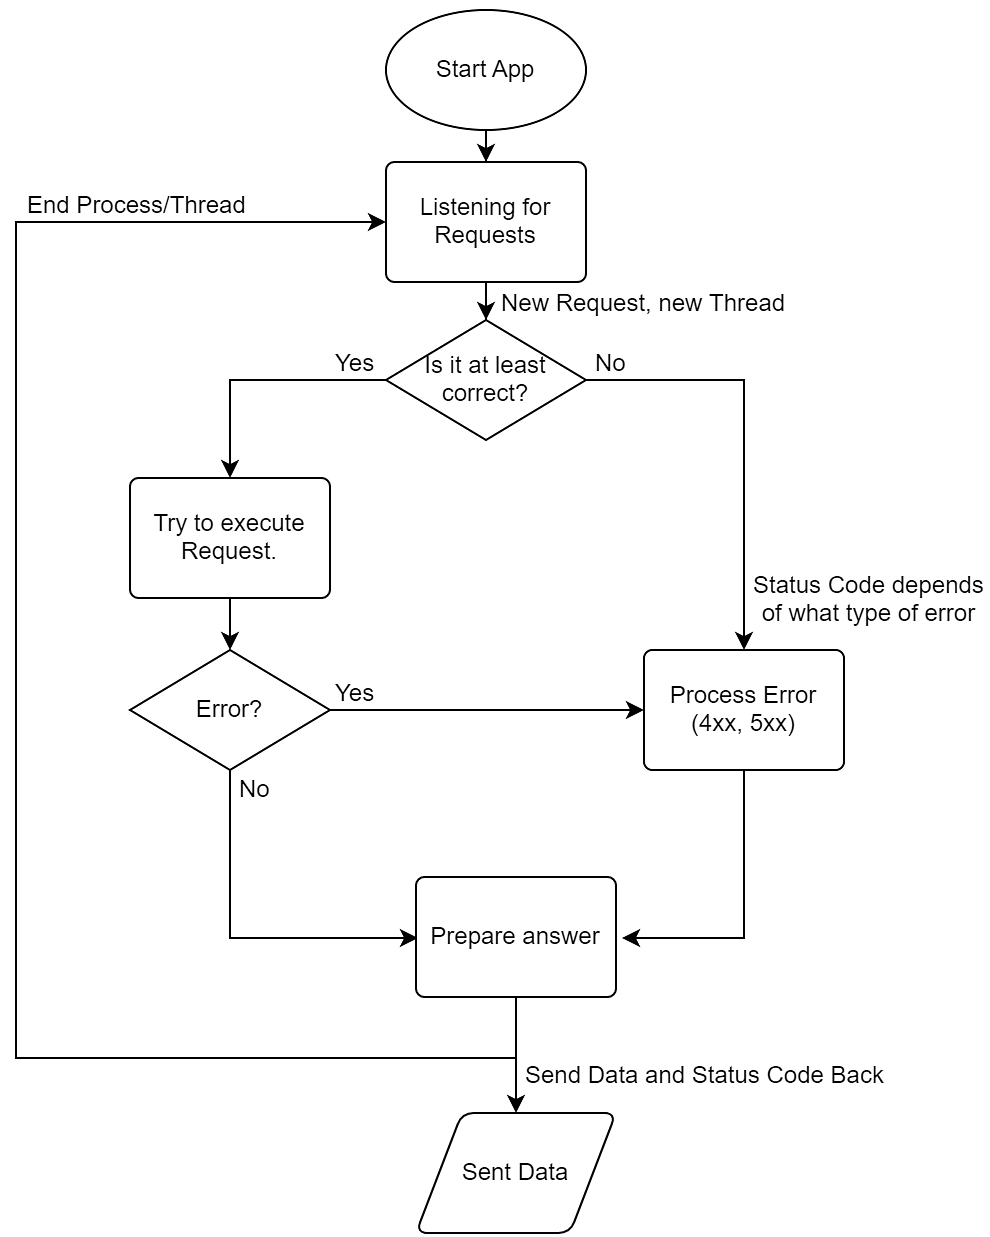
\includegraphics[width=14cm]{figuras/flowchart1.png}
        \caption{\textit{Flowchart} do funcionamento do microserviço, criado no \href{https://gitmind.com/app/flowchart/ccd11723910}{GitMind}}
        \label{fig:flow1}
\end{figure}
\FloatBarrier

Cada um destes processos descritos no \textit{flowchart} (os quadrados), é um objeto ou classe. Os principais vão ser seguidamente descritos com maior detalhe, nas secções seguintes.

\newpage

\section{Organização}

Este projeto (como anteriormente mencionado), é um projeto Gradle que contem dois subprojetos, os quais gerem tarefas diferentes mas co-dependentes:

\begin{itemize}
        \item O pacote dos \hyperref[endp]{\textit{Endpoints}}: um pacote para o core do projeto, este contem a estrutura MC do projeto, com os respectivos modelos, controller e o serviço que comunica com os repositórios do pacote seguinte;
        \item O pacote da \hyperref[infra]{\textit{Infrastructure}}: pacote para os repositórios que tratam das transações com a base de dados e as classes geradas do jOOQ que os repositórios utilizam.
\end{itemize}

Dentro da \textit{root directory} do projeto contemos variadas subdirectorias e ficheiros, dos quais podemos apontar:

\begin{itemize}
        \item \texttt{\textbf{build/ -> }} diretoria onde o Gradle gera os binários, os \textit{jars}, artefactos, etc\ldots da tarefa de compilação;
        \item \texttt{\textbf{endpoints/ -> }} \textit{source directory} do subprojeto \hyperref[endp]{\textit{Endpoints}};
        \item \texttt{\textbf{gradle/ -> }} diretoria onde existem os \textit{wrappers} do Gradle;
        \item \texttt{\textbf{infrastructure/ -> }} \textit{source directory} do subprojeto \hyperref[infra]{\textit{Infrastructure}};
        \item \texttt{\textbf{javadoc/ -> }} diretoria onde se gera o JavaDoc, ou seja um documento/\textit{website} com a documentação (derivada dos \textit{block comments});
        \item \texttt{\textbf{build.gradle -> }} ficheiro de configuração \textbf{principal} do Gradle, onde definimos os pacotes a ir buscar e programamamos as tarefas de (pré e pós) compilação e de testes;
        \item \texttt{\textbf{gradle.properties -> }} ficheiro de configuração \textbf{opcional} do Gradle onde se definem \textit{compiler flags}, argumentos para a JVM e outras configurações mais profundas e especificas;
        \item \texttt{\textbf{lombok.config -> }} ficheiro de configuração \textbf{opcional} do Lombok, onde aqui defino para adicionar a anotação \texttt{@Generated} as suas classes geradas para \textit{fugir} ao JaCoCo;
        \item \texttt{\textbf{micronaut-cli.yml -> }} ficheiro de preferências da criação de um projeto Micronaut via a sua ferramenta CLI;
        \item \texttt{\textbf{postgres-compose.yml -> }} ficheiro de \textbf{docker-compose} para compor e lançar containers com pré configurações, neste caso um container de PostgreSQL;
        \item \texttt{\textbf{settings.gradle -> }} ficheiro de configuração do Gradle onde se definem os subprojetos do projeto Gradle, é executado a cada \textit{build task}.
\end{itemize}

\newpage

\subsection{\textit{\textit{Endpoints} package}}\label{endp}

Este é o subprojeto \textit{Endpoints} onde contêm toda a estrutura base da API, deste o ponto inicial da aplicação, às configurações, modelos, controladores e serviços. Tendo em conta que \texttt{com/optiply/endpoint/} fica como reticências, temos que:

\begin{itemize}
        \item \texttt{\textbf{src/main/}}\begin{itemize}
                      \item \texttt{\textbf{java/}}\begin{itemize}
                                    \item \texttt{\textbf{\ldots/config/}}\begin{itemize}
                                                  \item \texttt{\textbf{DataSourceConfig.java}}
                                          \end{itemize}
                                    \item \texttt{\textbf{\ldots/controllers/}}\begin{itemize}
                                                  \item \texttt{\textbf{shared/interfaces/IBaseController.java}}
                                                  \item \texttt{\textbf{shared/BaseController.java}}
                                                  \item \texttt{\textbf{JSONController.java}}
                                          \end{itemize}
                                    \item \texttt{\textbf{\ldots/models/}}\begin{itemize}
                                                  \item \texttt{\textbf{EmailListModel.java}}
                                                  \item \texttt{\textbf{HandleModel.java}}
                                                  \item \texttt{\textbf{InterestRateModel.java}}
                                                  \item \texttt{\textbf{ServiceLevelsModel.java}}
                                                  \item \texttt{\textbf{SettingsModel.java}}
                                                  \item \texttt{\textbf{UrlModel.java}}
                                                  \item \texttt{\textbf{WebshopFullModel.java}}
                                                  \item \texttt{\textbf{WebshopModel.java}}
                                                  \item \texttt{\textbf{WebshopSettingsModel.java}}
                                          \end{itemize}
                                    \item \texttt{\textbf{\ldots/services/}}\begin{itemize}
                                                  \item \texttt{\textbf{RepositoryService.java}}
                                          \end{itemize}
                                    \item \texttt{\textbf{\ldots/EndpointApplication.java}}
                            \end{itemize}
                      \item \texttt{\textbf{resources/}}\begin{itemize}
                                    \item \texttt{\textbf{db/migration/}}\begin{itemize}
                                                  \item \texttt{\textbf{V1\_\_create\_initial\_schema.sql}}
                                          \end{itemize}
                                    \item \texttt{\textbf{application.yaml}}
                                    \item \texttt{\textbf{bootstrap.yaml}}
                                    \item \texttt{\textbf{logback.xml}}
                            \end{itemize}
              \end{itemize}
\end{itemize}

\newpage

\begin{itemize}
        \item \texttt{\textbf{src/test/}}\begin{itemize}
                      \item \texttt{\textbf{java/}}\begin{itemize}
                                    \item \texttt{\textbf{integration/}}\begin{itemize}
                                                  \item \texttt{\textbf{\ldots/controllers/JSONControllerIntegrationTests.java}}
                                          \end{itemize}
                                    \item \texttt{\textbf{shared/}}\begin{itemize}
                                                  \item \texttt{\textbf{\ldots/container/TestContainer.java}}
                                                  \item \texttt{\textbf{\ldots/environment/TestEnvironment.java}}
                                          \end{itemize}
                                    \item \texttt{\textbf{unit/}}\begin{itemize}
                                                  \item \texttt{\textbf{\ldots/models/WebshopFullModelsUnitTests.java}}
                                                  \item \texttt{\textbf{\ldots/services/RepositoryServiceUnitTests.java}}
                                          \end{itemize}
                            \end{itemize}
                      \item \texttt{\textbf{resources/}}\begin{itemize}
                                    \item \texttt{\textbf{application-test.yaml}}
                            \end{itemize}
              \end{itemize}
\end{itemize}

Sendo que é clara a funcionalidade de cada classe pelo nome e pelo local onde se encontra. Mesmo sendo esse o caso, seguimos para uma explicação breve do que cada classe ou ficheiro faz, excluindo as classes de modelos, pois são obviamente modelos dos objetos transacionais (os corpos em JSON do \textit{request} HTTP) ou de suas partes.

\subsubsection*{\texttt{DataSourceConfig.java}}

Esta classe executa o carregamento e pós-configuração das configurações do ficheiro de configuração \texttt{application.yaml}, criando o contexto DSL (uma interface de comunicação do jOOQ com a base de dados via JDBC), e consequentemente cria a \textit{ConnectionFactory}, que permite usar R2DBC e fazer queries transacionais de forma reactiva.

\subsubsection*{\texttt{JSONController.java}}

Esta classe é um controlador de \textit{requests} HTTP com \textit{payloads} em JSON. Esta, extende a classe de controlador base \texttt{BaseController.java} (abstrata), que por si é uma implementação da interface \texttt{IBaseController.java}, que contem as funções der \textit{parsing} dos parâmetros de procura e sorteamento do \textit{endpoint} de pesquisa de Webshops.

\subsubsection*{\texttt{RepositoryService.java}}

Esta classe é responsável por deter toda a \textit{business logic} necessária e acessível pelos \textit{controllers} e que os isola de contacto direto com os repositórios de dados. É aqui que se executam as tarefas que queremos executadas e recebemos os resultados quando usamos os \textit{endpoints} do \textit{controller}.

\newpage

\subsubsection*{\texttt{EndpointApplication.java}}

Classe principal/base de onde executa a aplicação.

\subsubsection*{\texttt{application.yaml}}

Ficheiro de configurações da aplicação (referido anteriormente \texttt{DataSourceConfig.java}). É aqui onde temos configurações da framework, como o uso do FlyWay, do jOOQ, configurações da fonte de dados (base de dados) e dos meios como lhe comunica (JDBC e R2DBC).

\subsubsection*{\texttt{application-test.yaml} \textsuperscript{\textit{Testes}}}

Semelhante ao anterior, em funcionalidade e não só em nome, são as configurações especificas a ser usadas quando executamos testes. Assim podendo escolher meios de segregar ambientes e containers de teste, ou ajustar recursos de sistema. Neste caso, foi para usar containers de teste novos por cada novo \textit{set} de testes, via TestContainers.

\subsubsection*{\texttt{TestContainer.java} \textsuperscript{\textit{Testes}}}

Classe que configura o lançamento de uma nova instância de um container PostgreSQL (sobre TestContainers) para ser usado como container de testes.

\subsubsection*{\texttt{TestEnvironment.java} \textsuperscript{\textit{Testes}}}

Classe que abstrai o funcionamento da classe anterior quando esta for instanciada qualquer classe de testes que a extenda. Sendo que todas as classes de testes extendem esta classe, ou seja, estão sobre o mesmo ambiente de testes.

\subsubsection*{\texttt{JSONControllerIntegrationTests.java} \textsuperscript{\textit{Testes}}}

Para fazer os testes de integração, testes que testam todo um funcionamento ou percurso não isolado de um processo do projeto, apenas precisamos de fazer testes ao \textit{controller}. Fazendo com que este esteja a receber pedidos HTTP e a escutar as respostas que ele dá, verificando se os resultados obtidos são os esperados.

\subsubsection*{\texttt{WebshopFullModelsUnitTests.java} \textsuperscript{\textit{Testes}}}

Qualquer processo que ocorra nesta aplicação, é um processo de \textit{messaging}, em que o conteúdo das mensagens é dados de um modelo ou o modelo em si, se queremos ter a certeza que estas mensagens ocorrem de forma esperada temos de testar os modelos que elas comunicam. Esta classe faz testes unitários a cada modelo incluso neste projeto.

\subsubsection*{\texttt{RepositoryServiceUnitTests.java} \textsuperscript{\textit{Testes}}}

O serviço neste projeto é o \textit{middleware} que ofusca o \textit{business logic}, como também serve como a comunicação entre os pontos de entrada e o repositório dados que contem o que é pedido, aqui estão definidos os fluxos reactivos das tarefas a fazer. É preciso fazer testes unitários a este serviço, usando o Mockito para imitar comportamentos de classes e objetos que este comunique para isolar o \textit{scope} dos testes.

\subsubsection*{\texttt{V1\_\_create\_initial\_schema.sql}}

Ficheiro \texttt{.sql} com o esquema inicial da base de dados, onde o Gradle executa uma tarefa com o pacote FlyWay para fazer a migração. Esta base de dados contêm duas tabelas, uma com Webshops e as suas caraterísticas e outra para os emails de contacto das Webshops, relação de um-para-muitos.

\subsection{\textit{\textit{Infrastructure} package}}\label{infra}

O subprojeto do \textit{Infrastructure} é onde toda a lógica de comunicação com a base de dados está instalada, desde as classes autogeradas do jOOQ aos repositórios, que são as classes que visam o isolamento e abstração das transações SQL com os que requerem que sejam executadas, nomeadamente o serviço no subprojeto anterior.

\begin{itemize}
        \item \texttt{\textbf{src/main/java/\ldots/data}}\begin{itemize}
                      \item \texttt{\textbf{repositories/}}\begin{itemize}
                                    \item \texttt{\textbf{interfaces/}}\begin{itemize}
                                                  \item \texttt{\textbf{IWebshopemailsRepository.java}}
                                                  \item \texttt{\textbf{IWebshopRepository.java}}
                                          \end{itemize}
                                    \item \texttt{\textbf{WebshopemailsRepository.java}}
                                    \item \texttt{\textbf{WebshopRepository.java}}
                            \end{itemize}
                      \item \texttt{\textbf{support/sql/}}\begin{itemize}
                                    \item \texttt{\textbf{QueryResult.java}}
                            \end{itemize}
                      \item \texttt{\textbf{package-info.java}}
                      \item \texttt{\textbf{resources/}}\begin{itemize}
                                    \item \texttt{\textbf{jooq\_schema.sql}}
                            \end{itemize}
              \end{itemize}
\end{itemize}

Aqui contem artefactos peculiares, dos quais interfaces para cada Repositório, uma classe de Enums, um ficheiro SQL e um \textit{package-info}. Estes vãos ser seguidamente explicados, tal como no capitulo anterior.

\newpage

\subsubsection*{\texttt{IWebshopRepository.java}}

Interface para implementação do repositório que faz as operações CRUD da tabela de Webshops. Esta interface permite ao Mockito interpretar o comportamento a imitar da classe \texttt{WebshopRepository}.

\subsubsection*{\texttt{IWebshopemailsRepository.java}}

Semelhante à anterior mas para a tabela de emails das Webshops.

\subsubsection*{\texttt{WebshopRepository.java}}

Classe de operações CRUD reactivas, esta é a classe usada pelo serviço quando necessita de fazer operações na tabela de Webshops.

\subsubsection*{\texttt{WebshopemailsRepository.java}}

Semelhante à anterior mas para operações na tabela de emails das Webshops.

\subsubsection*{\texttt{QueryResult.java}}

Enum de resultados das queries SQL, permitindo fazer operações de equivalência a \textit{result codes} e \textit{status}.

\subsubsection*{\texttt{jooq\_schema.sql}}

Ficheiro com o esquema da base de dados em SQl para que o jOOQ possa criar todas as classes e sistemas referentes à base de dados que é usada. Desde POJOs para usar como objetos transacionais como DAOs e \textit{Specific Result Sets}.

\subsubsection*{\texttt{package-info.java}}

Classe que é interpretada pela framework e que têm apenas como objetivo obrigar a que os parâmetros seja \textit{Nullable by default}. Esta configuração foi herdada pelo estado inicial do projeto.

\newpage

\section{Código}

Nesta seguinte secção vai ser vista em maior detalhe algumas classes e o seu funcionamento especifico, como também explicada algumas decisões po detrás das escolhas feitas sobre o que foi (e como foi) construído.

\subsection{\textit{JSON Controller}}

Esta classe de controlador extende o controlador base que por sí é uma implementação do da seguinte interface:

\begin{verbatim}
/**
 * Interface for a base controller.
 */
public interface IBaseController {
        
        /**
         * Parse params and return a condition.
         *
         * @param params the params
         * @return the condition
         */
        Condition parseParamsWebshop(String... params);
        
        /**
         * Sort parser for the webshops.
         *
         * @param sort  the sort
         * @param order the order
         * @return the sort field
         */
        SortField<?> sortParserWebshop(String sort, String order);
}
\end{verbatim}

Sendo que estes dois métodos são apenas precisos para a função de pesquisa, porém esta sendo um ponto crucial e também o mais importante do micro serviço, estará sempre como requerimento de qualquer possível implementação de um controlador, quer seja ele de \textit{requests} HTTP, gRPC ou quais quer outros.

O \texttt{parseParamsWebshop} faz a gestão de toas as condições exposats na URL de pesquisa, tais como \textit{``nome igual a''}, \textit{``nome semelhante a''} ou \textit{``taxa de juro maior/menor que''}. Já a \texttt{sortParserWebshop} indica qual a ordem de chegada dos resultados, sendo que podem de forma ascendente ou descendente (numérica ou alfa-numericamente), ser ordenados por quais quer das suas colunas.

As implementações desses métodos estão nos anexos \hyperref[an1]{um} e \hyperref[an2]{dois}. A classe implementação também Injeta dois objetos que qualquer classe extensa de esta base precisa: o acesso ao serviço e o \texttt{ObjectMapper} do Jackson.

\begin{verbatim}
 /**
 * The repository service.
 */
@Inject
public RepositoryService repositoryService;
/**
 * Jackson object mapper.
 */
@Inject
public ObjectMapper objectMapper;
\end{verbatim}

Em suma, este controlador funciona da seguinte forma:

\begin{table}[!hbt]
        \centering
        \begin{tabular}{ll}
                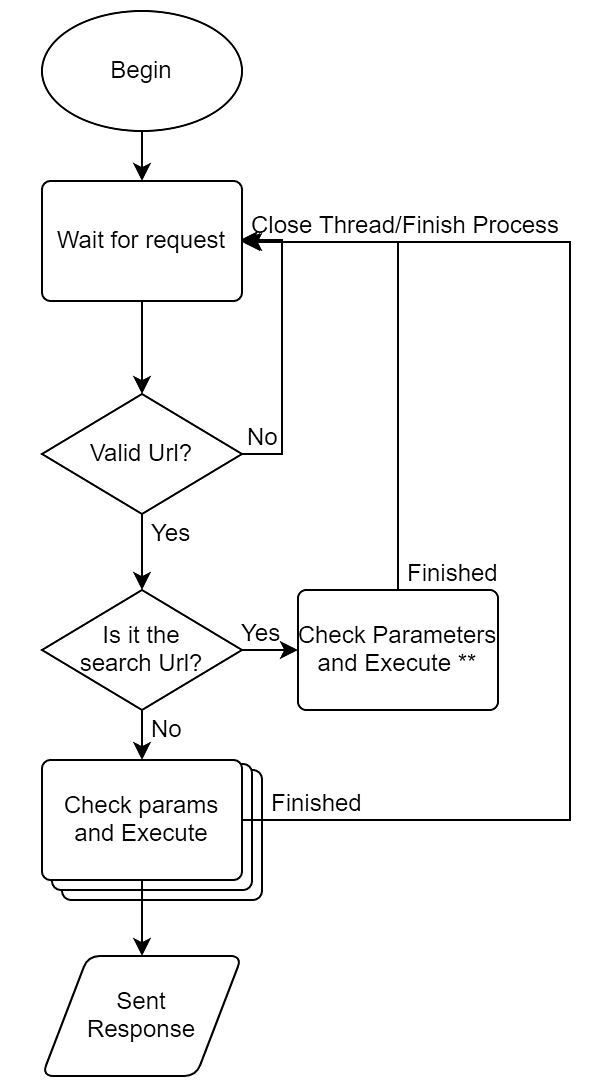
\includegraphics[width=6cm]{figuras/flowchart2.png}
                \label{fig:flow2} &
                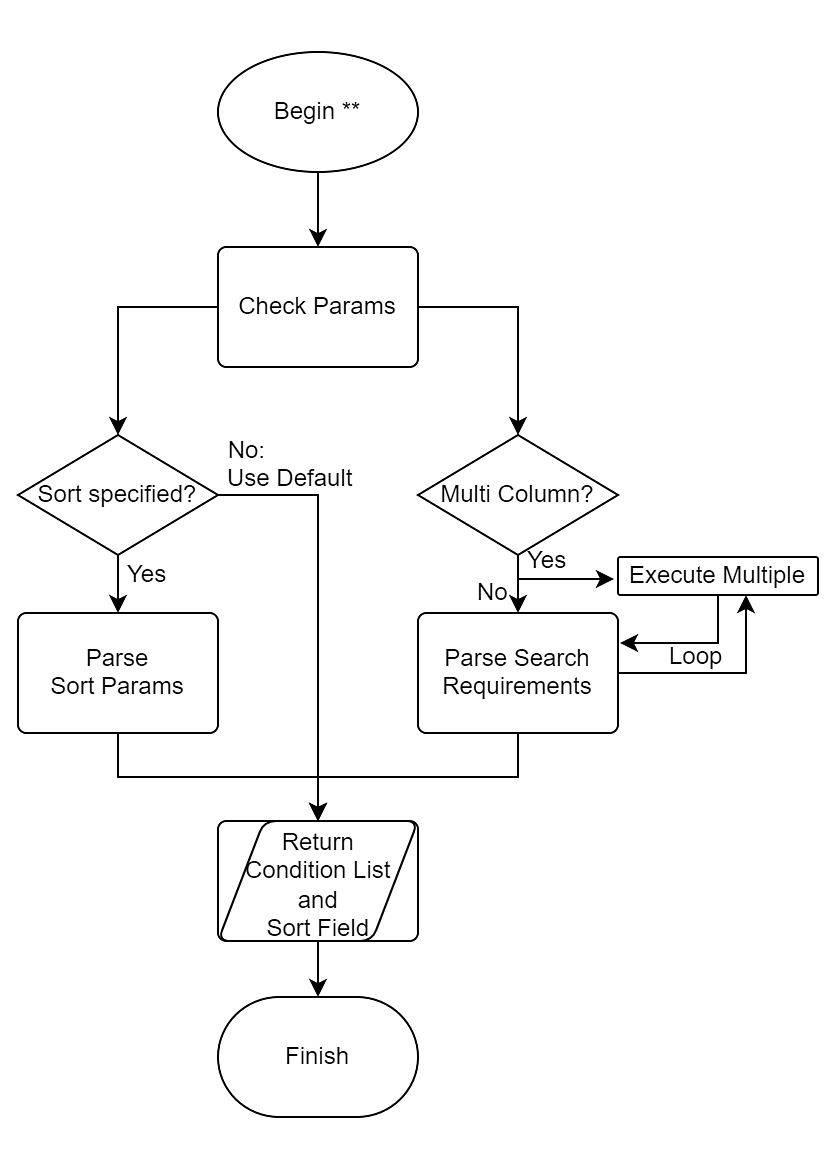
\includegraphics[width=7cm]{figuras/flowchart3.png}
                \label{fig:flow3}   \\
        \end{tabular}
        \caption{\textit{Flowchart} do funcionamento geral do controlador, criado no \href{https://gitmind.com/app/flowchart/8d511739737}{GitMind}}
\end{table}
\FloatBarrier

\newpage

\subsection{\textit{Webshop Service}}



\subsection{Modelos}

\subsubsection*{Modelos \textit{Webshop\ldots}}

\subsubsection*{Restantes modelos}

\subsection{Repositórios}

\subsubsection*{\texttt{WebshopRepository}}

\subsubsection*{\texttt{WebshopemailsRepository}}

\newpage
% para adicionar o  capítulo N adicione a linha \input{capituloN} e crie o ficheiro
% capituloN.tex na directoria "capitulos"

%%%%%%%%%%%%%%%%%%%%%%%%%%%%%%%%%%%%%%%%%%%%%%%%
% Bibliografia
\clearpage
\printbibliography[heading=bibintoc]
%%%%%%%%%%%%%%%%%%%%%%%%%%%%%%%%%%%%%%%%%%%%%%%%
\apendices
\chapter{Título do Apêndice I}
\label{ap1}

%a linha seguinte deve ser substituída pelo texto do apêndice
\lipsum
% para adicionar o  apêndice N adicione a linha \input{apendiceN} e crie o ficheiro
% apendiceN.tex na directoria "apendices"
%%%%%%%%%%%%%%%%%%%%%%%%%%%%%%%%%%%%%%%%%%%%%%%%
\anexos
\chapter{Implementação do \texttt{parseParamsWebshop}}\label{an1}

\lstinputlisting[frame=bt,language=java,caption={parseParamsWebshop()}]{listagens/parseParamsWebshop.java}
\chapter{Implementação do \texttt{sortParserWebshop}}\label{an2}

\begin{verbatim}
@Override
public SortField<?> sortParserWebshop(String sort, String order) {

	if (sort == null || sort.isEmpty()) {
		sort = "handle";
	}

	if (order == null || order.isEmpty()) {
		order = "asc";
	}

	sort = sort.toLowerCase();
	order = order.toLowerCase();

	switch (sort) {
		case "handle" -> {
			if (order.equals("asc")) {
				return Tables.WEBSHOP.HANDLE.asc();
			} else if (order.equals("desc")) {
				return Tables.WEBSHOP.HANDLE.desc();
			}
			return Tables.WEBSHOP.HANDLE.asc();
		}

		
		case "url" -> {
			if (order.equals("asc")) {
				return Tables.WEBSHOP.URL.asc();
			} else if (order.equals("desc")) {
				return Tables.WEBSHOP.URL.desc();
			}
			return Tables.WEBSHOP.URL.asc();
		}
		case "interestrate" -> {
			if (order.equals("asc")) {
				return Tables.WEBSHOP.INTEREST_RATE.asc();
			} else if (order.equals("desc")) {
				return Tables.WEBSHOP.INTEREST_RATE.desc();
			}
			return Tables.WEBSHOP.INTEREST_RATE.asc();
		}
		// To add more later
	}

	return Tables.WEBSHOP.HANDLE.asc();
}
\end{verbatim}
\chapter{Implementação do \texttt{RepositoryService}}\label{an3}

\begin{verbatim}
/**
 * Repository service (middleware to remove business logic from controller).
 */
public class RepositoryService {


	/**
	 * The Webshop repository.
	 */
	@Inject
	public WebshopRepository webshopRepository;
	/**
	 * The Webshopemails repository.
	 */
	@Inject
	public WebshopemailsRepository webshopemailsRepository;

	/**
	 * Finds webshops via a conditionally defined
   * query sorted by a defined sort field.
	 *
	 * @param condition the condition
	 * @param sortField the sort field
	 * @return the webshops
	 */
	public Mono<MutableHttpResponse<List<WebshopModel>>> 
    getWebshops(Condition condition, SortField<?> sortField) {

		return webshopRepository.findVarious(condition, sortField)
      .flatMapSequential(this::getWebshopPriv)
				.collectList().flatMap(webshops -> {
					if (webshops.isEmpty()) {
						return Mono.empty();
					}
					return Mono.just(HttpResponse.ok(webshops));
				}).switchIfEmpty(Mono.just(HttpResponse.notFound()))
				.onErrorReturn(HttpResponse.serverError());


	}

	/**
	 * Helper method for getWebshops(), works exaclty
   * like the getWebshop() method, but without the
	 * HttpResponse wrapping.
	 *
	 * @param handle the handle
	 * @return the webshop
	 */
	private Mono<WebshopModel> getWebshopPriv(String handle) {

		return webshopRepository.find(handle)
      .flatMap(webshop -> Mono.just(new WebshopModel(webshop)))
				.flatMap(webshopModel -> webshopemailsRepository.findEmails(handle)
						.flatMap(webshopemails -> {
							webshopModel.setEmails(webshopemails);
							return Mono.just(webshopModel);
						}).flatMap(Mono::just));
	}

	/**
	 * Gets webshop by handle.
	 *
	 * @param handle the handle
	 * @return the webshop
	 */
	public Mono<MutableHttpResponse<WebshopModel>> getWebshop(String handle) {

		return webshopRepository
      .find(handle).flatMap(webshop -> Mono.just(new WebshopModel(webshop)))
				.flatMap(webshopModel -> webshopemailsRepository.findEmails(handle)
						.flatMap(webshopemails -> {
							webshopModel.setEmails(webshopemails);
							return Mono.just(webshopModel);
						}).flatMap(webshopModelWithEmails ->
								Mono.just(HttpResponse.ok(webshopModelWithEmails))))
				.switchIfEmpty(Mono.just(HttpResponse.notFound()))
				.onErrorReturn(HttpResponse.serverError());
	}

	/**
	 * Gets webshop settings by handle.
	 *
	 * @param handle the handle
	 * @return the webshop settings
	 */
	public Mono<MutableHttpResponse<WebshopSettingsModel>>
    getWebshopSettings(String handle) {

		return webshopRepository.find(handle)
				.flatMap(webshop ->
						Mono.just(new WebshopSettingsModel(webshop)))
				.flatMap(webshopSettingsModel ->
						Mono.just(HttpResponse.ok(webshopSettingsModel)))
				.switchIfEmpty(Mono.just(HttpResponse.notFound()))
				.onErrorReturn(HttpResponse.serverError());

	}

	/**
	 * Creates a single webshop via a webshop full model (webshop model + settings).
	 *
	 * @param webshopModel the webshop model
	 * @return the mono
	 */
	public Mono<MutableHttpResponse<String>>
    createWebshop(WebshopFullModel webshopModel) {

		if (!webshopModel.isValid()) {
			return Mono.just(HttpResponse.badRequest());
		}

		return webshopRepository.create(
						webshopModel.getHandle(), webshopModel.getUrl(),
						webshopModel.getServiceLevelA(), webshopModel.getServiceLevelB(),
            webshopModel.getServiceLevelC(), webshopModel.getInterestRate(),
            webshopModel.getCurrency(), webshopModel.getRunJobs(),
            webshopModel.getMultiSupplier()
				).flatMap(webshopResponse -> {
					if (webshopResponse) {
						return webshopemailsRepository
              .createVarious(webshopModel.getHandle(), webshopModel.getEmails())
								.flatMap(emailsResponse -> {
									if (emailsResponse) {
										return Mono.just(HttpResponse.ok("Webshop created."));
									}
									return Mono.empty();
								});
					}
					return Mono.empty();
				}).switchIfEmpty(Mono.just(HttpResponse.notFound()))
				.onErrorReturn(HttpResponse.serverError());
	}

	/**
	 * Creates various webshops via a list of
   * webshop full models (webshop model + settings).
	 *
	 * @param webshopModels the webshop models
	 * @return the mono
	 */
	public Mono<MutableHttpResponse<String>>
    createWebshops(List<WebshopFullModel> webshopModels) {

		for (WebshopFullModel webshopFullModel : webshopModels) {
			if (!webshopFullModel.isValid()) {
				return Mono.just(HttpResponse.badRequest());
			}
		}

		return Mono.just(webshopModels)
      .publishOn(Schedulers.boundedElastic()).flatMap(webshops -> {
					if (webshops.isEmpty()) {
						return Mono.empty();
					}
					for (WebshopFullModel webshopModel : webshops) {
						webshopRepository.create(
										webshopModel.getHandle(), webshopModel.getUrl(),
										webshopModel.getServiceLevelA(), webshopModel.getServiceLevelB(),
                    webshopModel.getServiceLevelC(), webshopModel.getInterestRate(),
                    webshopModel.getCurrency(),	webshopModel.getRunJobs(),
                    webshopModel.getMultiSupplier()
								).subscribeOn(Schedulers.boundedElastic())
								.then(webshopemailsRepository
                .createVarious(webshopModel.getHandle(), webshopModel.getEmails()))
								.subscribe();
					}
					return Mono.just(HttpResponse.ok("Webshops created."));
				}).switchIfEmpty(Mono.just(HttpResponse.badRequest()))
				.onErrorReturn(HttpResponse.serverError());

	}

	/**
	 * Deletes a single webshop by handle.
	 *
	 * @param handle the handle
	 * @return the mono
	 */
	public Mono<MutableHttpResponse<Object>> deleteWebshop(String handle) {

		return webshopRepository.deleteWebshop(handle).flatMap(response -> {
					if (response) {
						return Mono.just(HttpResponse.noContent());
					}
					return Mono.empty();
				}).switchIfEmpty(Mono.just(HttpResponse.badRequest()))
				.onErrorReturn(HttpResponse.serverError());
	}


	/**
	 * Fully updates a single webshop by getting the webshop full model.
	 *
	 * @param handle       the handle
	 * @param webshopModel the webshop model
	 * @return the mono
	 */
	public Mono<MutableHttpResponse<String>>
    updateWebshop(String handle, WebshopFullModel webshopModel) {

		return webshopRepository.updateWebshop(handle, webshopModel.getHandle(),
						webshopModel.getUrl(), webshopModel.getServiceLevelA(),
						webshopModel.getServiceLevelB(), webshopModel.getServiceLevelC(),
						webshopModel.getInterestRate(), webshopModel.getCurrency(),
						webshopModel.getRunJobs(), webshopModel.getMultiSupplier()
				).flatMap(response -> {
					if (response) {
						return webshopemailsRepository.deleteAll(webshopModel.getHandle())
								.flatMap(deleteResponse ->
										webshopemailsRepository.createVarious(webshopModel.getHandle(),
                      webshopModel.getEmails())
												.flatMap(emailsResponse -> {
													if (emailsResponse) {
														return Mono.just(HttpResponse.ok("Webshop updated."));
													}
													return Mono.just(HttpResponse
                            .ok("Webshop updated without emails."));
												}));
					}
					return Mono.empty();
				}).switchIfEmpty(Mono.just(HttpResponse.notFound()))
				.onErrorReturn(HttpResponse.serverError());
	}

	/**
	 * Updates a single webshop's handle.
	 *
	 * @param handle    the handle
	 * @param newHandle the new handle
	 * @return the mono
	 */
	public Mono<MutableHttpResponse<String>>
    updateWebshopHandle(String handle, String newHandle) {

		return webshopRepository.updateWebshopHandle(handle, newHandle)
				.flatMap(response -> {
					if (response) {
						return Mono.just(HttpResponse.ok("Webshop updated."));
					}
					return Mono.empty();
				}).switchIfEmpty(Mono.just(HttpResponse.notFound()))
				.onErrorReturn(HttpResponse.serverError());
	}

	/**
	 * Updates a single webshop's url.
	 *
	 * @param handle the handle
	 * @param url    the url
	 * @return the mono
	 */
	public Mono<MutableHttpResponse<String>>
    updateWebshopUrl(String handle, String url) {

		return webshopRepository.updateWebshopUrl(handle, url)
				.flatMap(response -> {
					if (response) {
						return Mono.just(HttpResponse.ok("Webshop updated."));
					}
					return Mono.empty();
				}).switchIfEmpty(Mono.just(HttpResponse.notFound()))
				.onErrorReturn(HttpResponse.serverError());
	}


	/**
	 * Updates a single webshop's interest rate.
	 *
	 * @param handle       the handle
	 * @param interestRate the interest rate
	 * @return the mono
	 */
	public Mono<MutableHttpResponse<String>>
    updateWebshopInterestRate(String handle, Short interestRate) {

		return webshopRepository.updateWebshopInterestRate(handle, interestRate)
				.flatMap(response -> {
					if (response) {
						return Mono.just(HttpResponse.ok("Webshop updated."));
					}
					return Mono.empty();
				}).switchIfEmpty(Mono.just(HttpResponse.notFound()))
				.onErrorReturn(HttpResponse.serverError());
	}


	/**
	 * Updates a single webshop's settings.
	 *
	 * @param handle        the handle
	 * @param settingsModel the webshop settings model
	 * @return the mono
	 */
	public Mono<MutableHttpResponse<String>>
    updateWebshopSettings(String handle, SettingsModel settingsModel) {

		return webshopRepository.updateWebshopSettings(handle,
						settingsModel.getCurrency(), settingsModel.getRunJobs(),
						settingsModel.getMultiSupplier())
				.flatMap(response -> {
					if (response) {
						return Mono.just(HttpResponse.ok("Webshop updated."));
					}
					return Mono.empty();
				}).switchIfEmpty(Mono.just(HttpResponse.notFound()))
				.onErrorReturn(HttpResponse.serverError());
	}


	/**
	 * Updates a single webshop's service levels.
	 *
	 * @param handle             the handle
	 * @param serviceLevelsModel the webshop service levels model
	 * @return the mono
	 */
	public Mono<MutableHttpResponse<String>> updateWebshopServiceLevels
	(String handle, ServiceLevelsModel serviceLevelsModel) {

		return webshopRepository.updateWebshopServiceLevels(
						handle, serviceLevelsModel.getServiceLevelA(),
						serviceLevelsModel.getServiceLevelB(),
            serviceLevelsModel.getServiceLevelC())
				.flatMap(response -> {
					if (response) {
						return Mono.just(HttpResponse.ok("Webshop updated."));
					}
					return Mono.empty();
				}).switchIfEmpty(Mono.just(HttpResponse.notFound()))
				.onErrorReturn(HttpResponse.serverError());
	}


	/**
	 * Updates a single webshop's emails.
	 *
	 * @param handle      the handle
	 * @param emailsModel the emails model
	 * @return the mono
	 */
	public Mono<MutableHttpResponse<String>>
    updateWebshopEmails(String handle, EmailListModel emailsModel) {

		return webshopemailsRepository.updateWebshopEmails(handle,
			emailsModel.getEmails())
				.flatMap(response -> {
					if (response) {
						return Mono.just(HttpResponse.ok("Webshop emails updated."));
					}
					return Mono.empty();
				}).switchIfEmpty(Mono.just(HttpResponse.notFound()))
				.onErrorReturn(HttpResponse.serverError());
	}
}
\end{verbatim}
% para adicionar o  anexo N adicione a linha \input{anexoN} e crie o ficheiro
% anexoN.tex na directoria "anexos"
%%%%%%%%%%%%%%%%%%%%%%%%%%%%%%%%%%%%%%%%%%%%%%%%
\end{document}
